%Template da SBC para artigos em português

\documentclass[12pt]{article}

\usepackage{sbc-template}
\usepackage{graphicx,url}
\usepackage[utf8]{inputenc}
\usepackage[brazil]{babel}
%\usepackage[latin1]{inputenc}  

\usepackage{longtable}
\usepackage{tabularx}
\usepackage{array}
\usepackage{booktabs}
\usepackage{float}

    
\sloppy

\title{AgroSys: Sistema de Gestão Agrícola}

\author{Fernanda Vitória Araújo Santos}

\address{
  Curso de Análise e Desenvolvimento de Sistemas -- Instituto Federal do Piauí (IFPI)\\
  Picos, PI -- Brasil
  \email{fernandacomun@gmail.com}
}

\begin{document}

\maketitle


\begin{resumo}
  O AgroSys é um sistema web de gestão agrícola desenvolvido para auxiliar pequenos produtores rurais na organização de suas atividades. O sistema permite gerenciar plantações, colheitas, estoque de insumos, vendas e tarefas agrícolas por meio de uma API REST e uma interface web moderna. O projeto busca melhorar o planejamento da produção, reduzir perdas de informação e facilitar a tomada de decisões através da centralização dos dados agrícolas.
\end{resumo}


\section{Visão Geral}

A gestão eficiente das atividades agrícolas é essencial para garantir uma produção organizada e sustentável. Entretanto, muitos pequenos produtores rurais ainda realizam o controle de suas informações de forma manual, utilizando cadernos, anotações ou planilhas, o que dificulta o acompanhamento da produção e o planejamento das atividades da propriedade.

\subsection{Problema}

Muitos produtores rurais, especialmente os pequenos produtores, enfrentam dificuldades para controlar informações importantes, como:

\begin{itemize}
  \item Plantações cadastradas;
  \item Datas de plantio e previsão de colheita;
  \item Quantidade produzida;
  \item Estoque de insumos agrícolas;
  \item Registro de vendas realizadas;
  \item Atividades e tarefas pendentes na propriedade.
\end{itemize}

A descentralização dessas informações pode ocasionar perdas de dados, desperdício de recursos, dificuldades na organização das atividades e prejuízos financeiros, além de comprometer o planejamento das próximas safras.

\subsection{Solução}

Com o objetivo de minimizar esses problemas, foi desenvolvido o \textbf{AgroSys}, um sistema web de gestão agrícola composto por uma API REST e uma interface web responsiva. A aplicação permite que produtores rurais centralizem as informações da propriedade em um único ambiente, facilitando o gerenciamento das principais atividades do dia a dia.

O sistema disponibiliza funcionalidades para o cadastro e acompanhamento de plantações, controle do estoque, gerenciamento de tarefas e registro de vendas, proporcionando uma visão organizada da produção.

O sistema busca oferecer uma solução simples, intuitiva e de fácil utilização, contribuindo para uma melhor organização da propriedade rural e auxiliando os produtores na tomada de decisões por meio de informações atualizadas e centralizadas.


\section{Descrição do Sistema}
O \textbf{AgroSys} é um sistema web desenvolvido para auxiliar pequenos produtores rurais no gerenciamento das atividades agrícolas de forma simples e centralizada. A aplicação foi projetada seguindo uma arquitetura cliente-servidor, sendo composta por um frontend responsável pela interface com o usuário e uma API REST responsável pelo processamento das regras de negócio e pela comunicação com o banco de dados.

O acesso ao sistema é realizado por meio de autenticação utilizando JSON Web Tokens (JWT), garantindo que apenas usuários autenticados possam acessar suas informações. Após o login, o usuário tem acesso aos módulos da aplicação, podendo cadastrar, consultar, atualizar e remover dados relacionados à sua propriedade.

\subsection{Funcionalidades}
O \textbf{AgroSys} disponibiliza os seguintes módulos:

\begin{itemize}
  \item \textbf{Gerenciamento de Plantações:} permite cadastrar culturas, informar datas de plantio e colheita, variedade cultivada, quantidade plantada, produção esperada, status da plantação e observações.

  \item \textbf{Controle de Estoque:} possibilita o cadastro e gerenciamento dos insumos e produtos armazenados, incluindo quantidade disponível, categoria, unidade de medida e preço unitário.

  \item \textbf{Gerenciamento de Vendas:} permite registrar as vendas realizadas, armazenando informações como cliente, data da venda, forma de pagamento, valor total e os produtos comercializados.

  \item \textbf{Gerenciamento de Tarefas:} possibilita criar, acompanhar e concluir atividades relacionadas à produção agrícola, auxiliando no planejamento das operações da propriedade.

  \item \textbf{Autenticação de Usuários:} realiza o cadastro, autenticação e gerenciamento das sessões dos usuários por meio de Access Tokens e Refresh Tokens.
\end{itemize}


\subsection{Fluxo de Funcionamento}

O fluxo de funcionamento do \textbf{AgroSys} inicia-se com o acesso do usuário à aplicação. Caso ainda não possua uma conta, é possível realizar o cadastro informando os dados necessários. Em seguida, o usuário efetua o login, enviando suas credenciais para a API REST.

A API valida as informações fornecidas e, quando a autenticação é realizada com sucesso, gera um \textit{Access Token} e um \textit{Refresh Token}. Esses tokens são utilizados para controlar o acesso às rotas protegidas do sistema e garantir que apenas usuários autenticados possam manipular seus dados.

Após a autenticação, o usuário é direcionado ao painel principal (\textit{Dashboard}), onde pode acessar os módulos disponíveis da aplicação. Entre as funcionalidades oferecidas estão o gerenciamento de plantações, controle de estoque, registro de vendas e gerenciamento de tarefas.

As operações realizadas em qualquer um desses módulos são enviadas ao backend por meio de requisições HTTP para a API REST. Antes de persistir as informações, a API realiza validações dos dados recebidos e aplica as regras de negócio definidas pelo sistema. Em seguida, os dados são armazenados no banco de dados PostgreSQL.

Após a conclusão da operação, a API retorna uma resposta ao frontend contendo o resultado da requisição. A interface é então atualizada, permitindo que o usuário visualize imediatamente as alterações realizadas.

A Figura~\ref{fig:fluxo} apresenta o fluxograma simplificado do funcionamento do \textbf{AgroSys}.

\begin{figure}[H]
  \centering
  \includegraphics[width=0.9\textwidth]{fluxo.png}
  \caption{Fluxo de funcionamento do AgroSys.}
  \label{fig:fluxo}
\end{figure}


\section{Interface do Sistema}

A interface do \textbf{AgroSys} foi desenvolvida com o objetivo de proporcionar uma experiência simples, intuitiva e responsiva aos pequenos produtores rurais. O frontend foi implementado utilizando Next.js, React, TypeScript e Tailwind CSS, priorizando uma navegação clara entre os módulos do sistema e facilitando o acesso às principais funcionalidades.

As telas foram organizadas de forma que o usuário consiga realizar suas operações com poucos passos, reduzindo a complexidade das tarefas diárias relacionadas ao gerenciamento da propriedade rural. Nesta seção são apresentadas as principais interfaces desenvolvidas.

\subsection{Tela de Login}

A autenticação é realizada por meio de credenciais cadastradas pelo usuário. Após a validação das informações na API REST, utilizando JSON Web Tokens (JWT), o acesso às funcionalidades do sistema é liberado.

\begin{figure}[H]
  \centering
  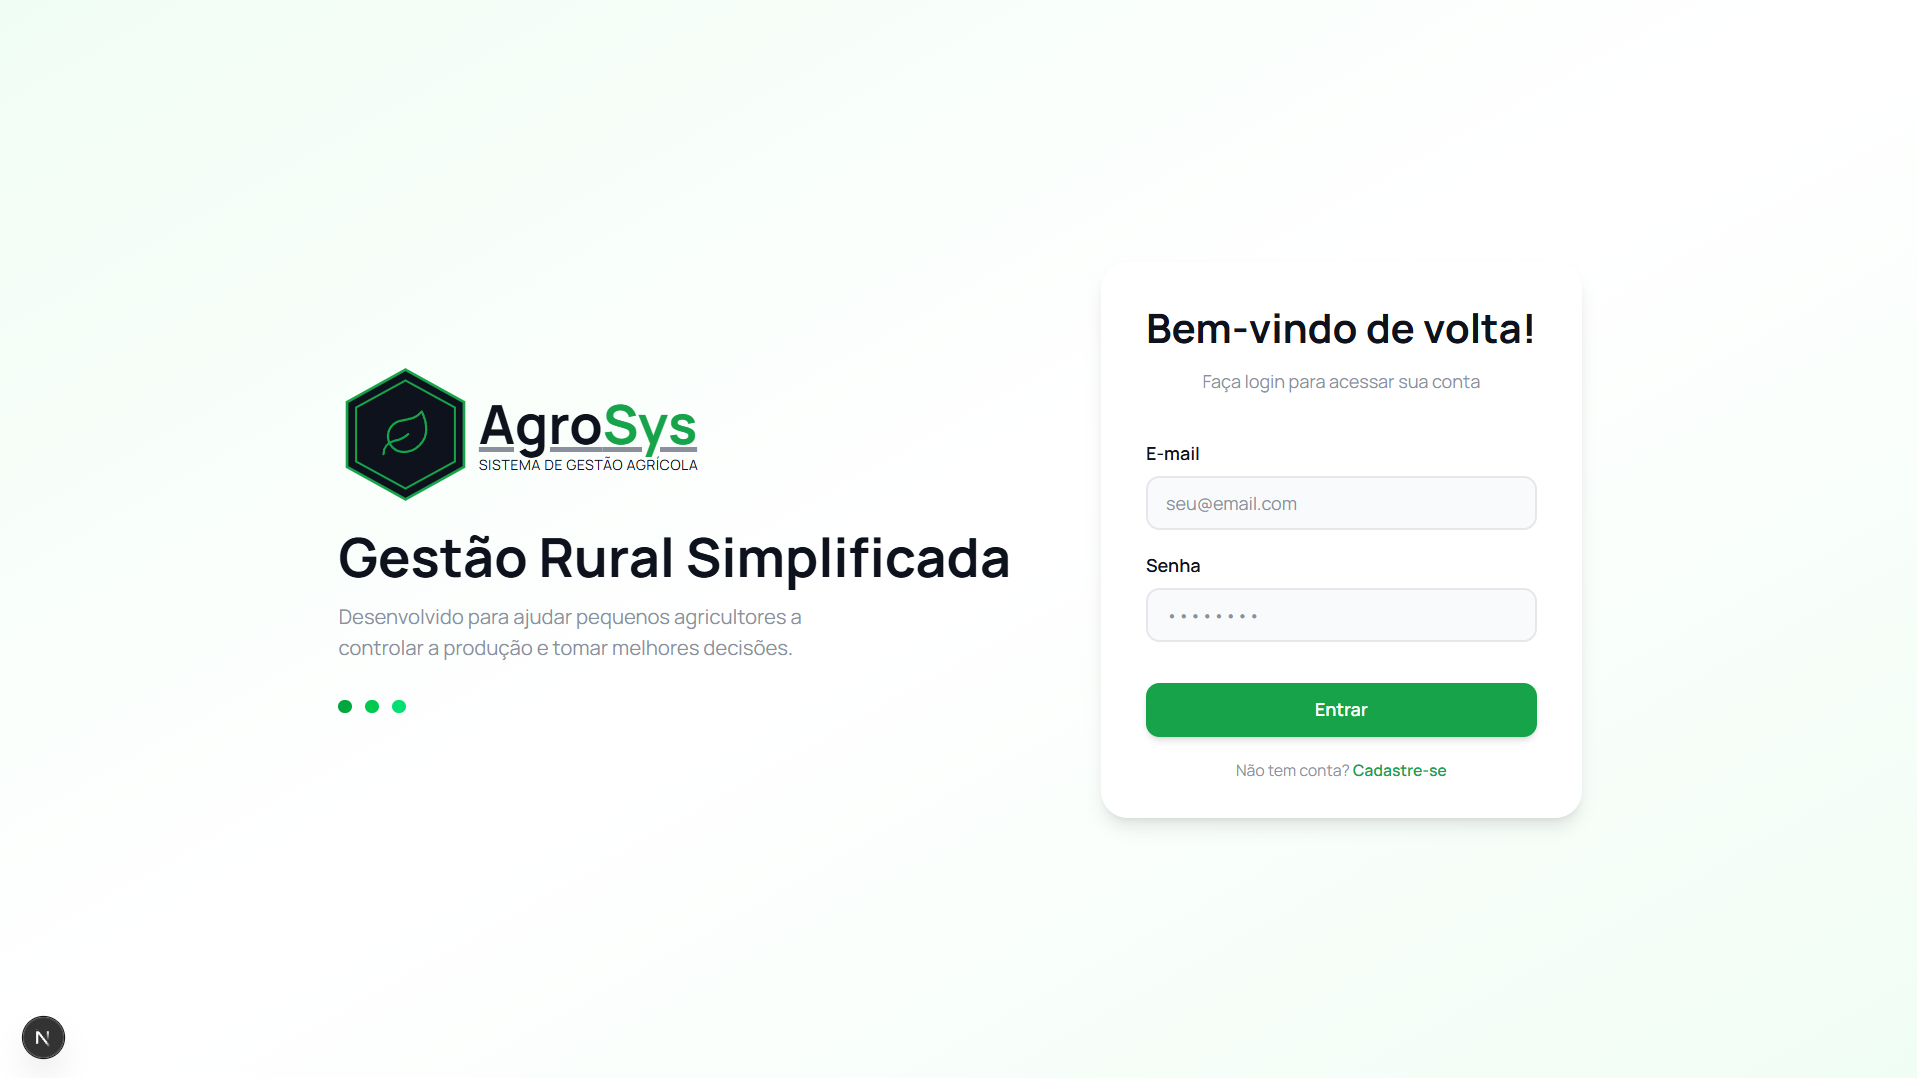
\includegraphics[width=0.9\textwidth]{login.png}
  \caption{Tela de autenticação do AgroSys.}
  \label{fig:login}
\end{figure}

\subsection{Dashboard}

Após a autenticação, o usuário é direcionado ao painel principal da aplicação. O dashboard reúne indicadores gerais do sistema, permitindo uma visão rápida das plantações cadastradas, tarefas pendentes e demais informações importantes para o gerenciamento da propriedade.

\begin{figure}[H]
  \centering
  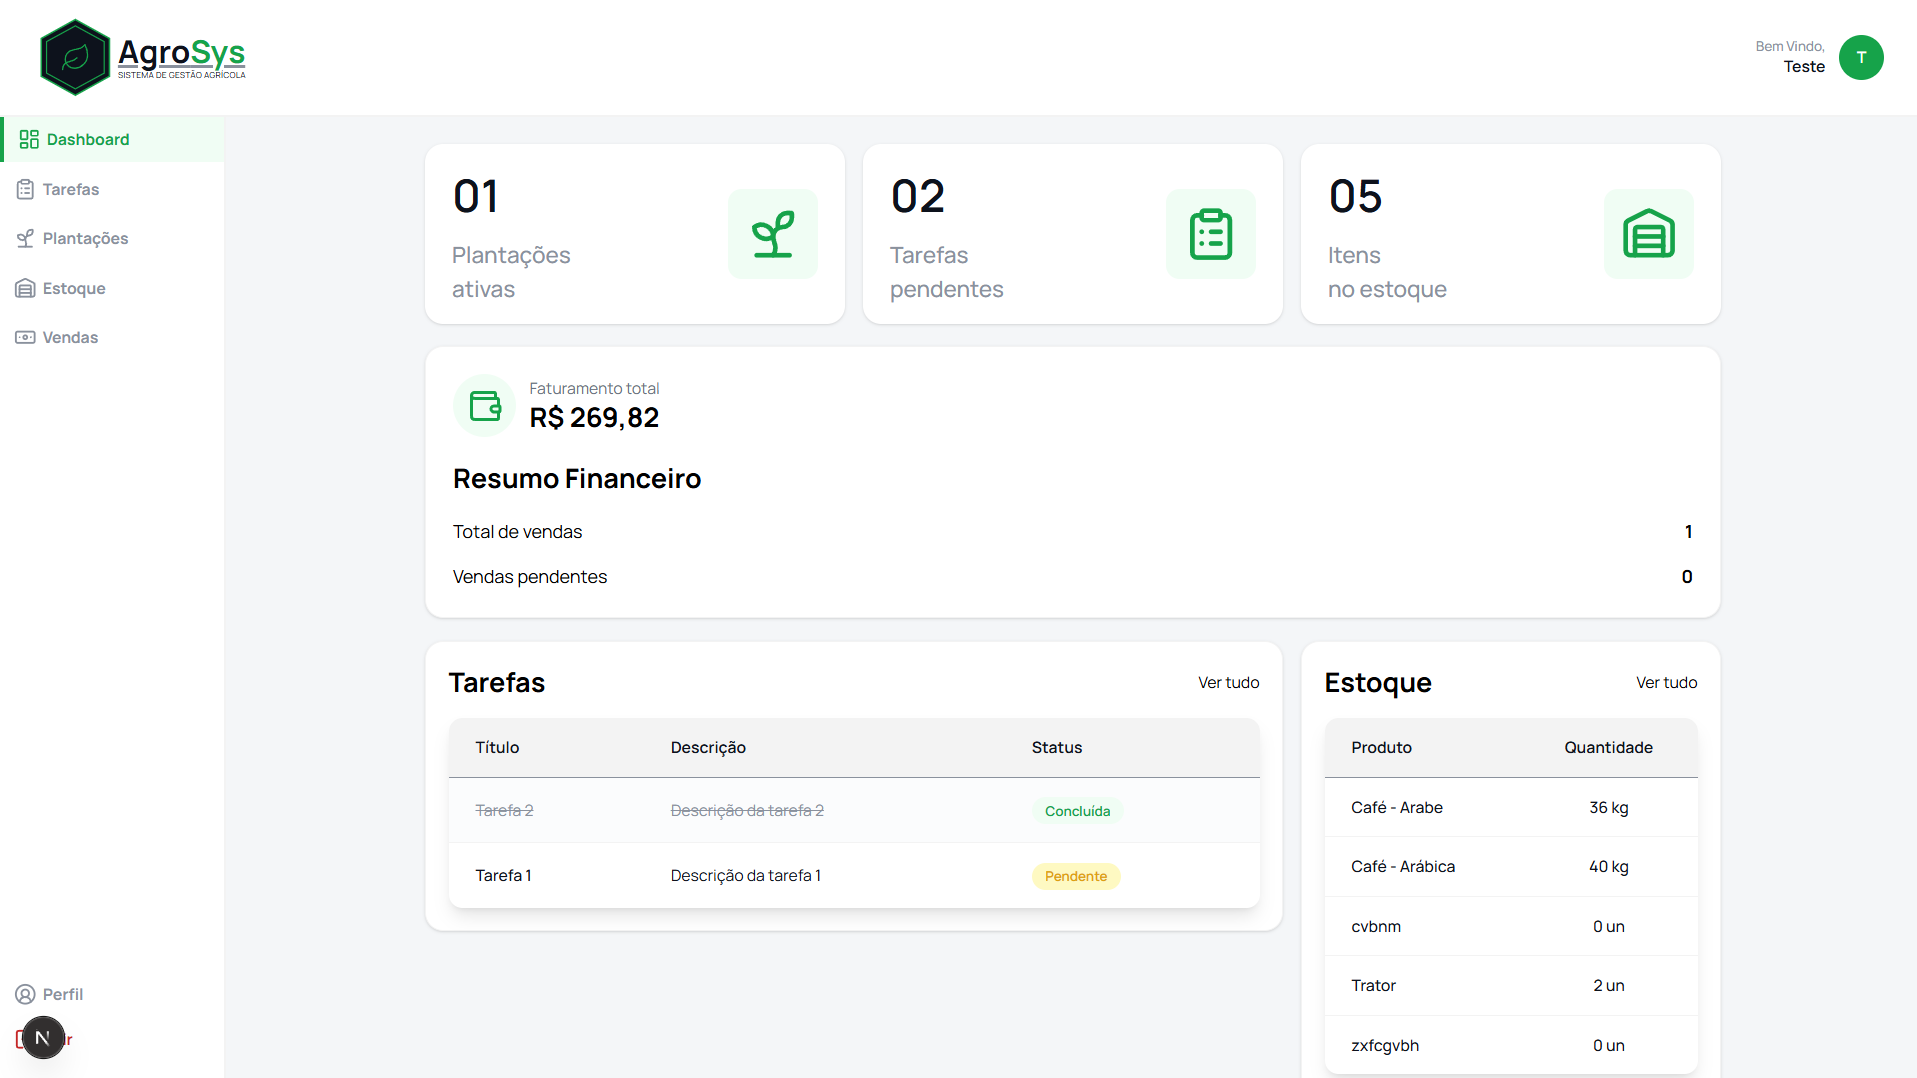
\includegraphics[width=0.9\textwidth]{dashboard.png}
  \caption{Painel principal do AgroSys.}
  \label{fig:dashboard}
\end{figure}

\subsection{Gerenciamento de Plantações}

O módulo de plantações permite cadastrar novas culturas, atualizar informações, acompanhar o status da produção e visualizar todas as plantações registradas pelo usuário.

\begin{figure}[H]
  \centering
  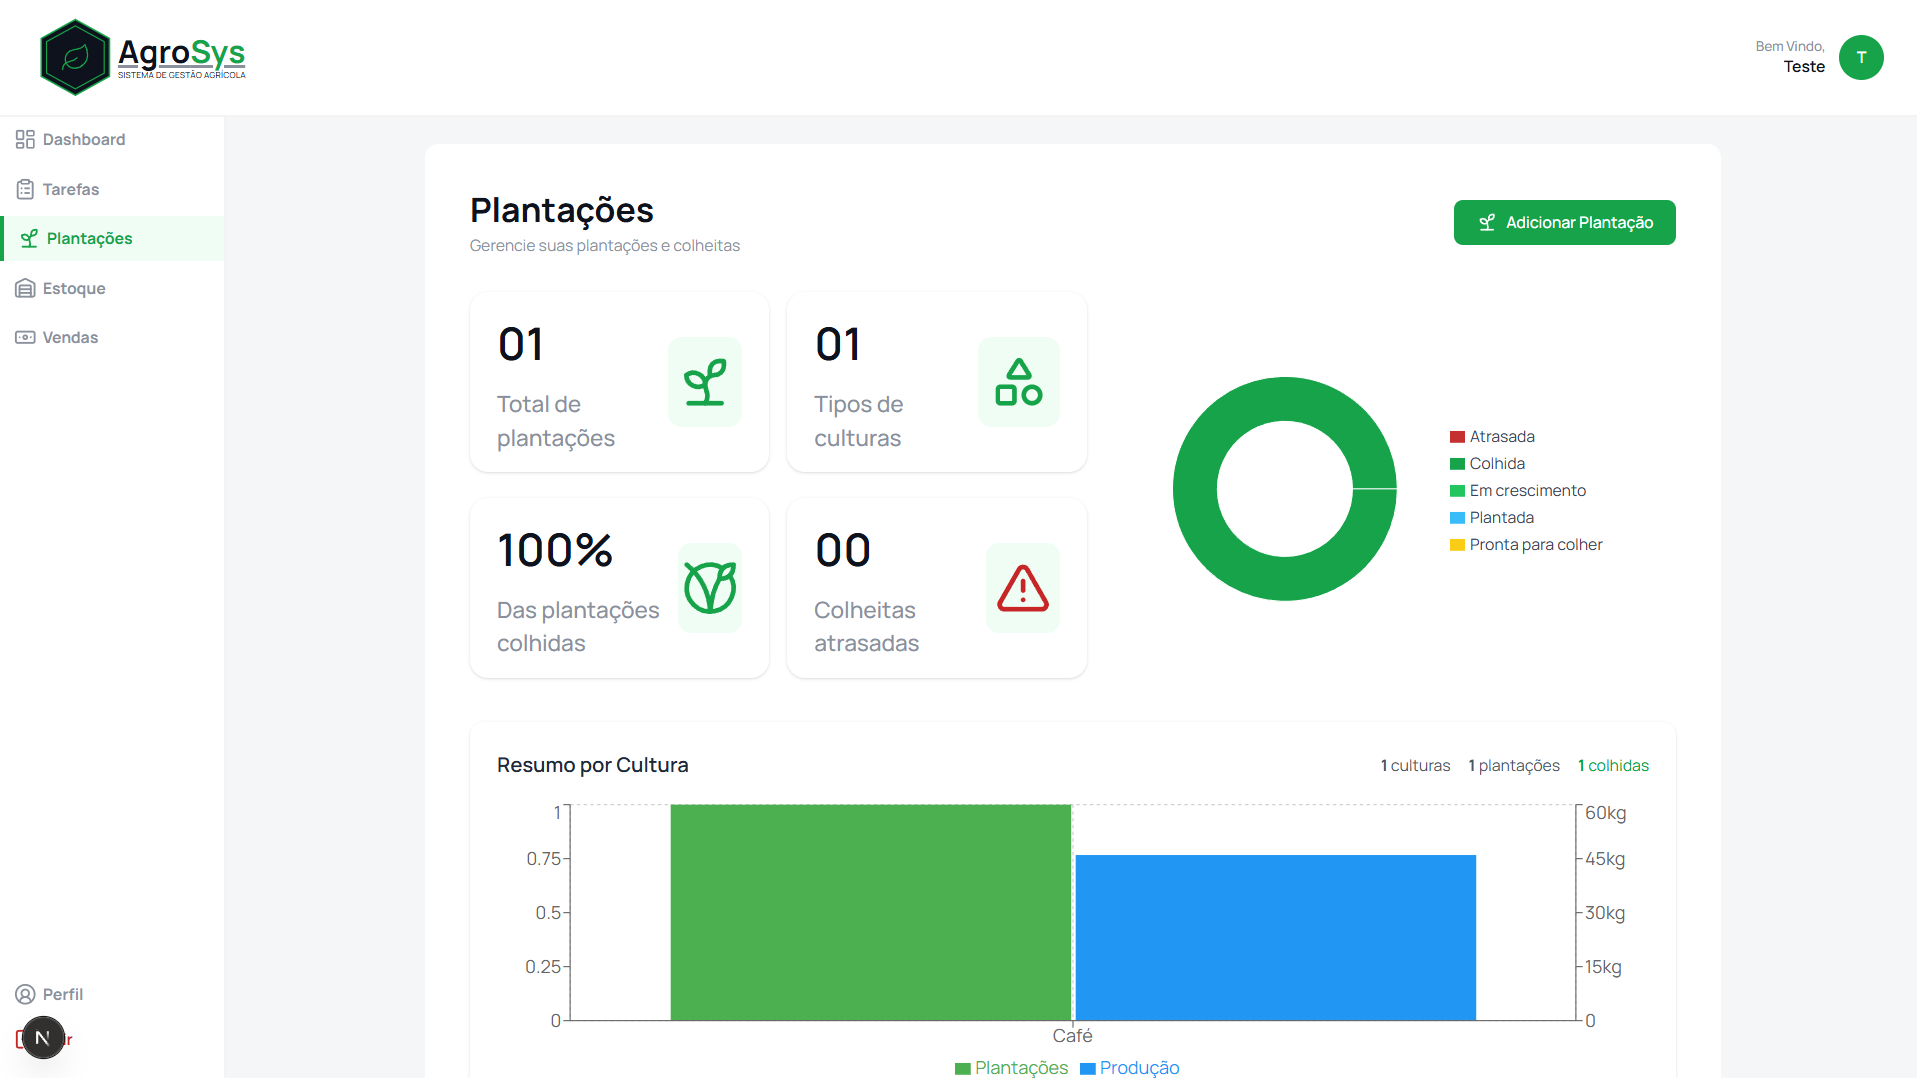
\includegraphics[width=0.9\textwidth]{plantacoes-1.png}
  \caption{Interface de gerenciamento de plantações.}
  \label{fig:plantacoes-1}
\end{figure}

\begin{figure}[H]
  \centering
  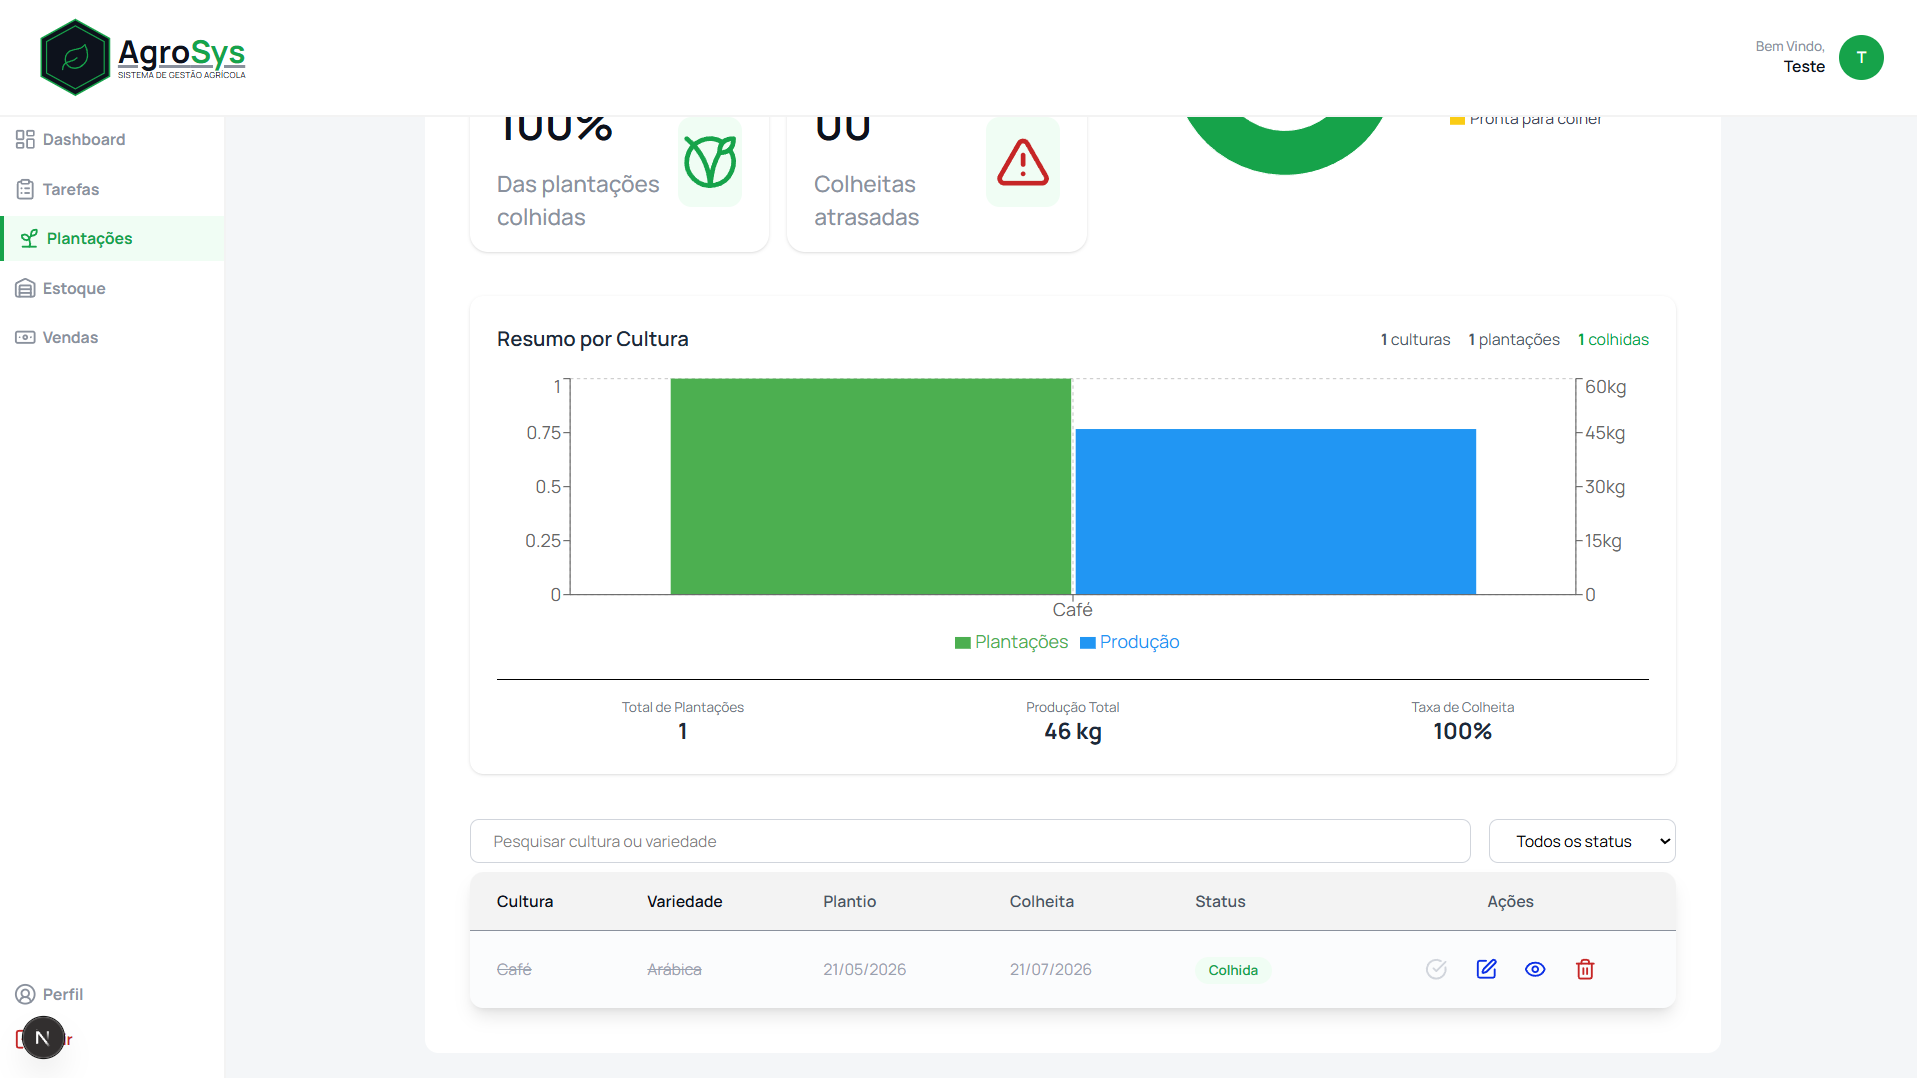
\includegraphics[width=0.9\textwidth]{plantacoes-2.png}
  \caption{Interface de gerenciamento de plantações.}
  \label{fig:plantacoes-2}
\end{figure}

\subsection{Controle de Estoque}

O gerenciamento de estoque possibilita controlar os produtos armazenados na propriedade, registrando quantidade disponível, categoria, unidade de medida e preço unitário.

\begin{figure}[H]
  \centering
  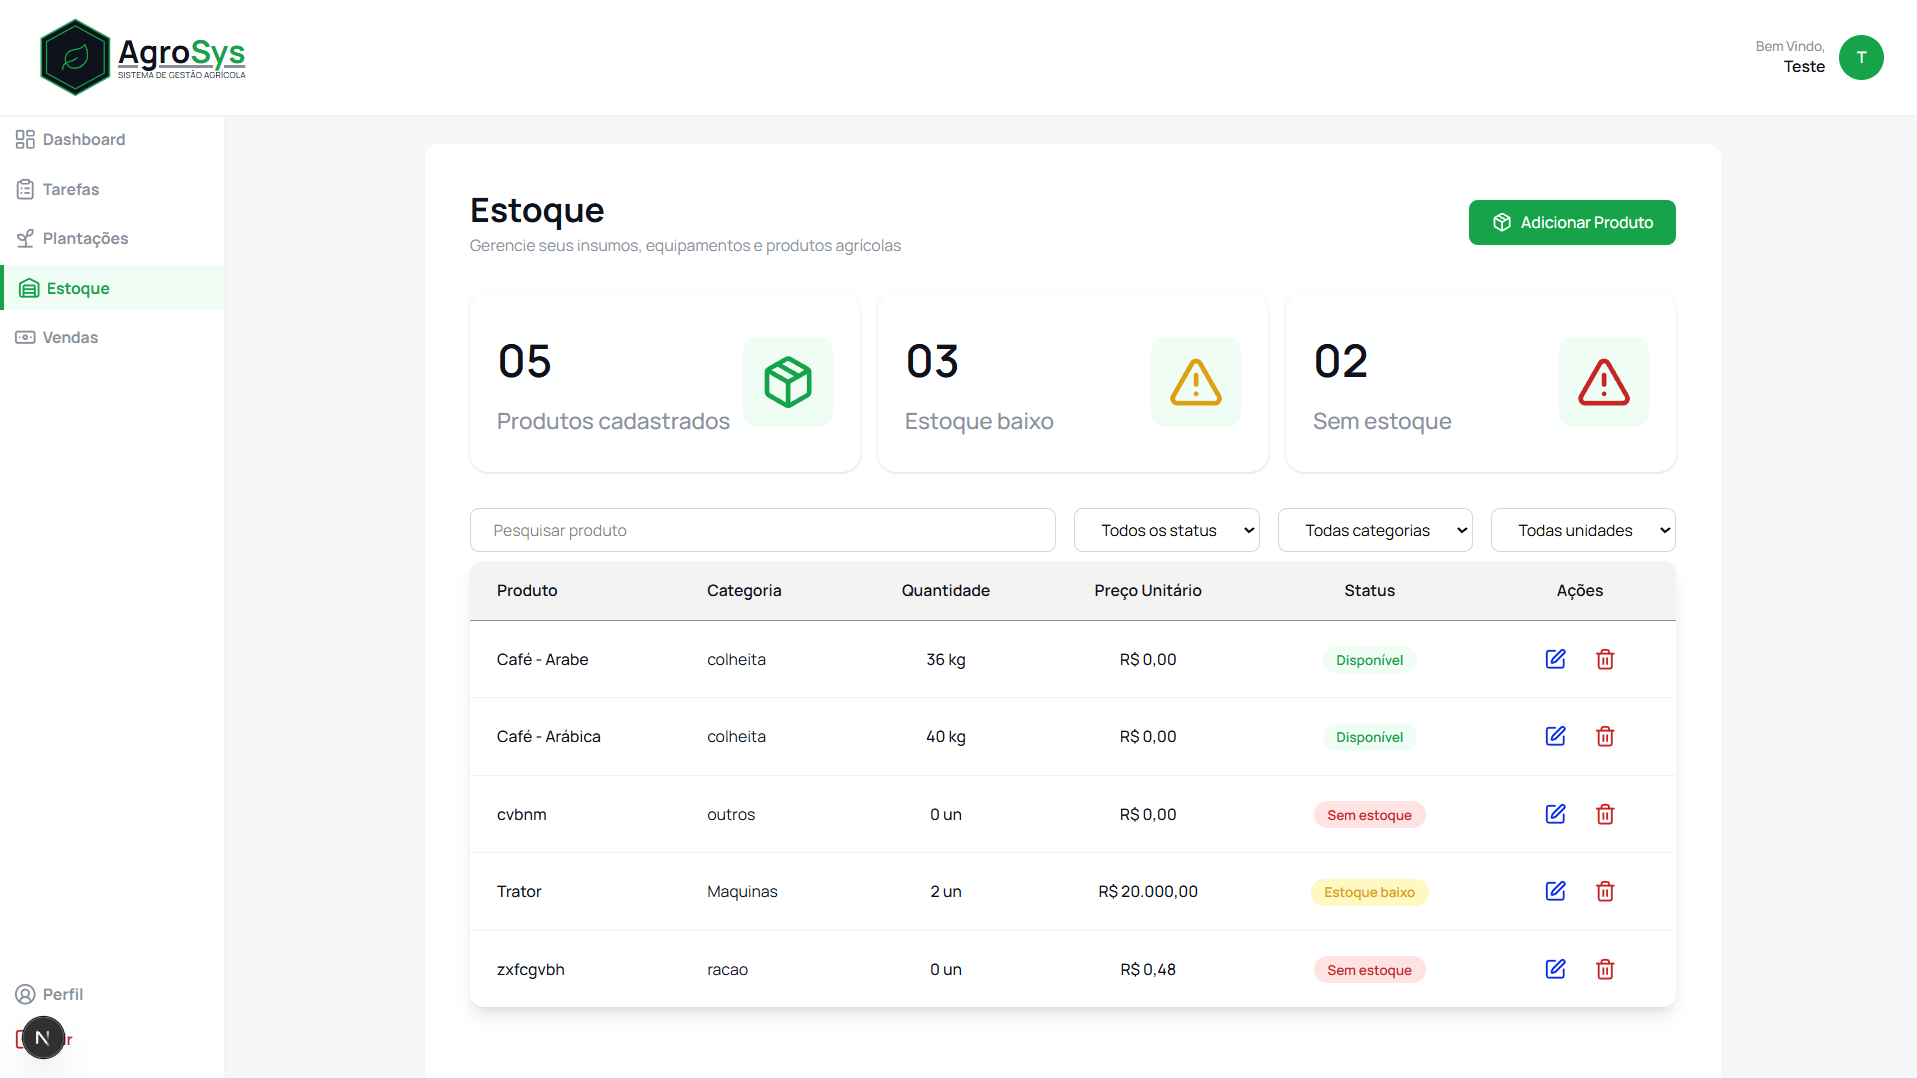
\includegraphics[width=0.9\textwidth]{estoque.png}
  \caption{Interface de gerenciamento de estoque.}
  \label{fig:estoque}
\end{figure}

\subsection{Gerenciamento de Vendas}

O módulo de vendas permite registrar comercializações realizadas, armazenando informações como cliente, forma de pagamento, produtos vendidos e valor total da operação.

\begin{figure}[H]
  \centering
  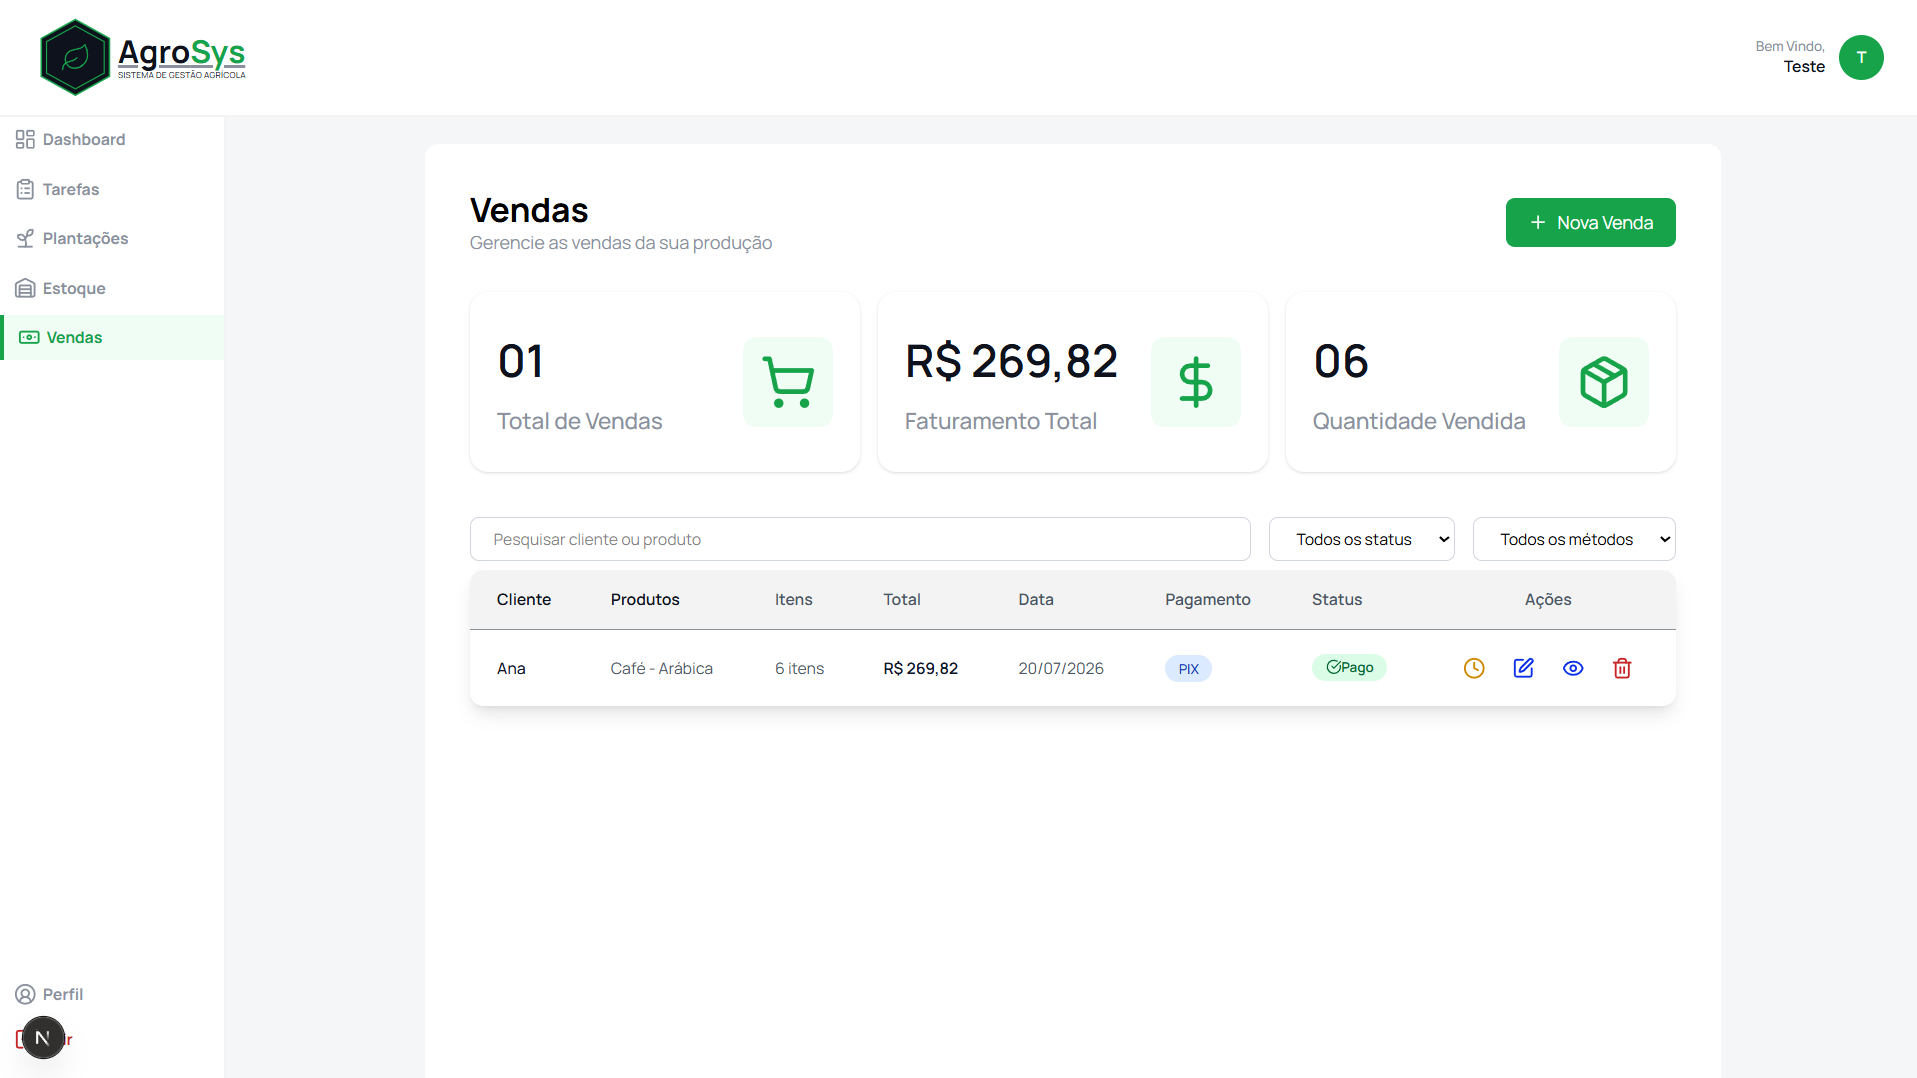
\includegraphics[width=0.9\textwidth]{vendas.png}
  \caption{Interface de gerenciamento de vendas.}
  \label{fig:vendas}
\end{figure}

\subsection{Gerenciamento de Tarefas}

O gerenciamento de tarefas auxilia no planejamento das atividades agrícolas, permitindo cadastrar, acompanhar e concluir atividades relacionadas à produção.

\begin{figure}[H]
  \centering
  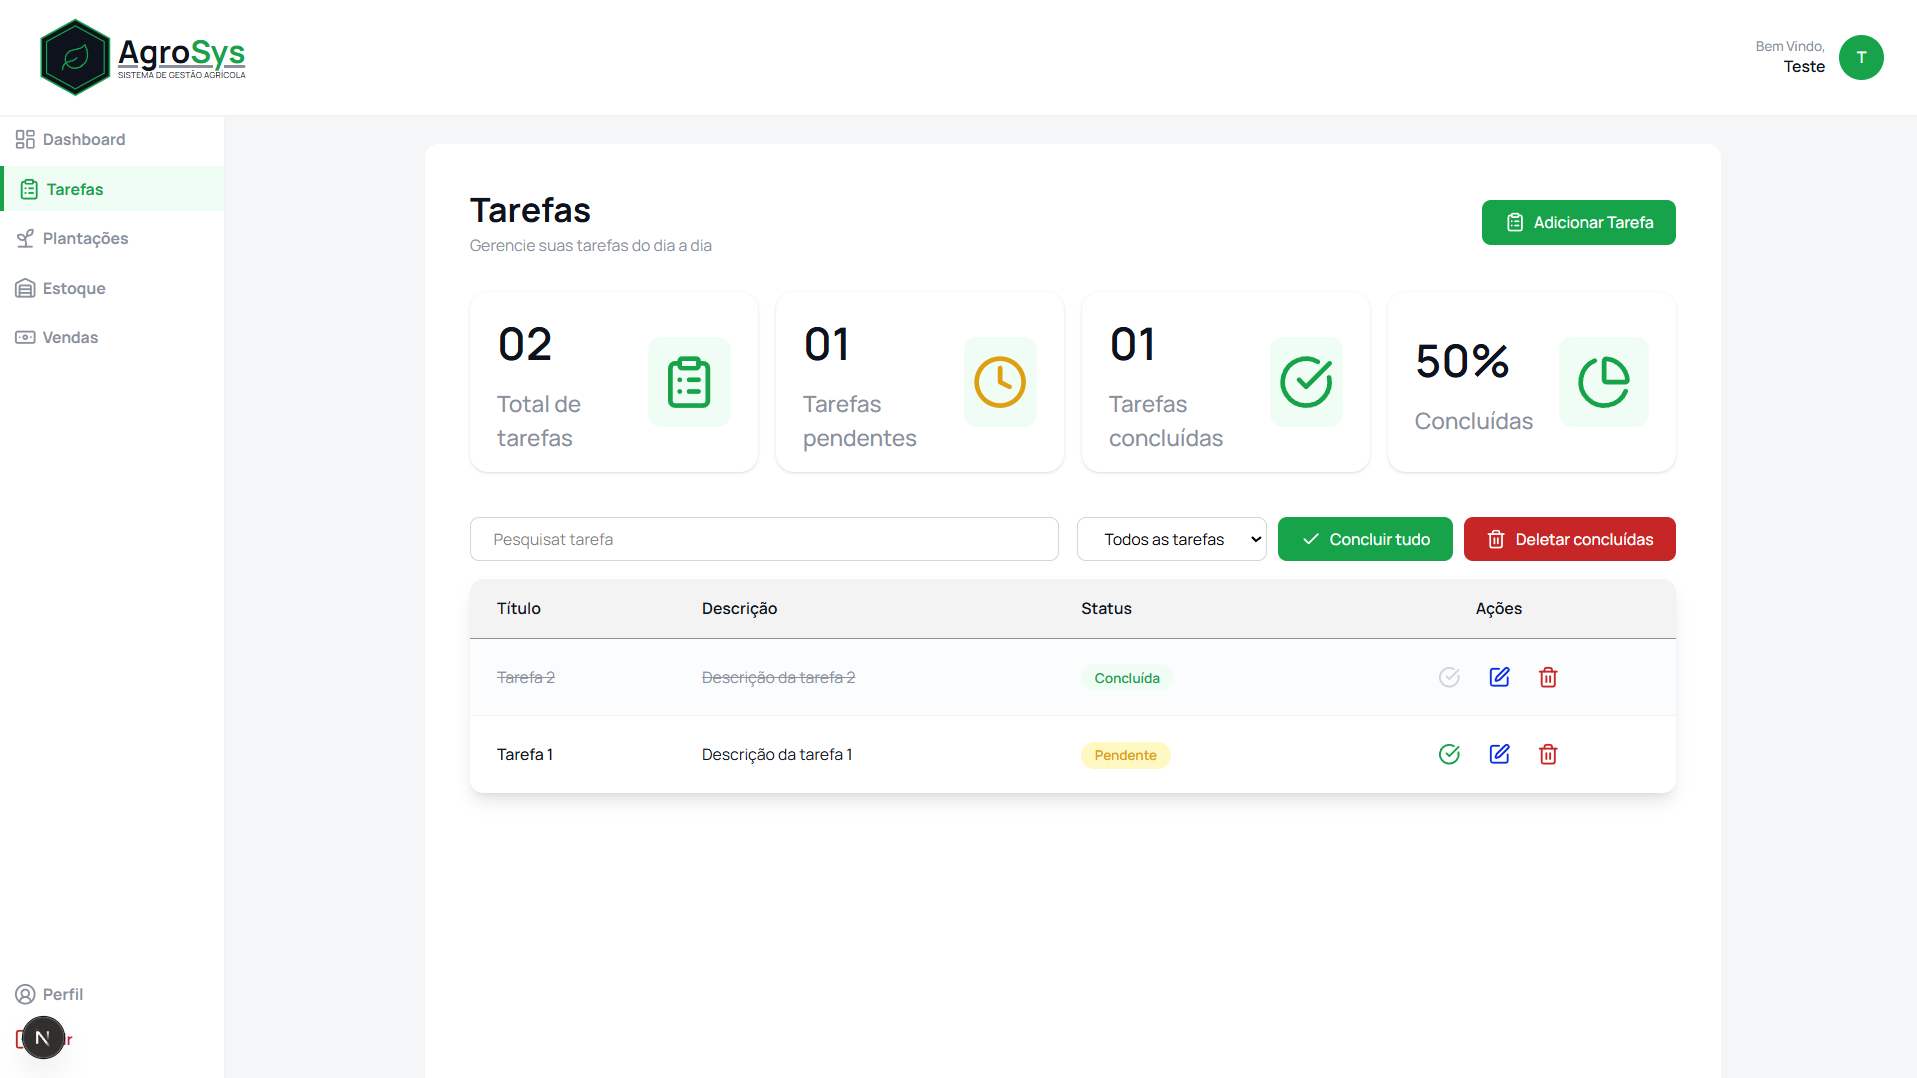
\includegraphics[width=0.9\textwidth]{tarefas.png}
  \caption{Interface de gerenciamento de tarefas.}
  \label{fig:tarefas}
\end{figure}


\section{Requisitos Funcionais}

O AgroSys foi desenvolvido para atender às principais necessidades relacionadas ao gerenciamento de propriedades rurais de pequeno porte. A Tabela~\ref{tab:rf} apresenta os principais requisitos funcionais implementados.

\begin{table}[H]
  \centering
  \caption{Requisitos funcionais do sistema}
  \label{tab:rf}

  \begin{tabular}{|c|p{10cm}|}
    \hline
    \textbf{Código} & \textbf{Descrição}                      \\ \hline
    RF01            & Permitir o cadastro de usuários.        \\ \hline
    RF02            & Permitir autenticação utilizando JWT.   \\ \hline
    RF03            & Cadastrar, editar e excluir plantações. \\ \hline
    RF04            & Gerenciar o estoque agrícola.           \\ \hline
    RF05            & Registrar vendas realizadas.            \\ \hline
    RF06            & Gerenciar tarefas agrícolas.            \\ \hline
    RF07            & Visualizar indicadores no Dashboard.    \\ \hline
  \end{tabular}

\end{table}

\section{Arquitetura do Projeto}

O \textbf{AgroSys} foi desenvolvido seguindo uma arquitetura cliente-servidor baseada no padrão de arquitetura em camadas, promovendo a separação entre a interface do usuário, as regras de negócio e a persistência dos dados. Essa organização facilita a manutenção do sistema, a reutilização de componentes e a escalabilidade da aplicação.

A arquitetura é composta por três camadas principais: frontend, backend e banco de dados. O frontend, desenvolvido com Next.js, React e TypeScript, é responsável por fornecer uma interface intuitiva e responsiva, permitindo que os usuários interajam com as funcionalidades do sistema.

O backend foi implementado utilizando Node.js e Express, disponibilizando uma API REST responsável por receber as requisições do frontend, realizar validações, aplicar as regras de negócio, controlar a autenticação dos usuários por meio de JSON Web Tokens (JWT) e acessar os dados armazenados no banco de dados.

A camada de persistência utiliza o PostgreSQL como sistema gerenciador de banco de dados relacional. A comunicação entre a aplicação e o banco é realizada por meio do Sequelize, que simplifica a manipulação das entidades utilizando o paradigma de Mapeamento Objeto-Relacional (ORM).

A comunicação entre o frontend e o backend ocorre por meio de requisições HTTP utilizando o formato JSON. Cada operação realizada pelo usuário, como cadastro de plantações, atualização do estoque, registro de vendas ou gerenciamento de tarefas, resulta em uma requisição à API, que processa a solicitação e retorna uma resposta para atualização da interface.

A Figura~\ref{fig:arquitetura} apresenta a arquitetura geral do \textbf{AgroSys}.

\begin{figure}[H]
  \centering
  \includegraphics[width=0.95\textwidth]{arquitetura.png}
  \caption{Arquitetura geral do AgroSys.}
  \label{fig:arquitetura}
\end{figure}


\section{Tecnologias Utilizadas}
\subsection{Backend}

\begin{longtable}{|p{3cm}|p{4.2cm}|p{7cm}|}
  \hline
  \textbf{Tecnologia}                                    & \textbf{Descrição} & \textbf{Finalidade no projeto}  \\
  \hline
  \endfirsthead

  \hline
  \textbf{Tecnologia}                                    & \textbf{Descrição} & \textbf{Finalidade no projeto}  \\
  \hline
  \endhead

  Node.js                                                &
  Ambiente de execução JavaScript no lado do servidor    &
  Desenvolvimento da API backend responsável pelas regras de negócio, autenticação e gerenciamento de usuários. \\
  \hline

  Express.js                                             &
  Framework para criação de aplicações web em Node.js    &
  Gerenciamento das rotas, requisições HTTP, middlewares e estrutura da API.                                    \\
  \hline

  Sequelize                                              &
  ORM (Object-Relational Mapping) para Node.js           &
  Modelagem das entidades e comunicação com o banco de dados utilizando modelos JavaScript.                     \\
  \hline

  dotenv                                                 &
  Biblioteca para gerenciamento de variáveis de ambiente &
  Armazenamento seguro de configurações sensíveis, como chaves JWT e dados de conexão com o banco.              \\
  \hline

  Nodemon                                                &
  Ferramenta de desenvolvimento                          &
  Reinicialização automática do servidor durante alterações no código.                                          \\
  \hline

  REST API                                               &
  Arquitetura de comunicação baseada no protocolo HTTP   &
  Comunicação entre cliente e servidor utilizando métodos como GET, POST, PUT e DELETE.                         \\
  \hline
\end{longtable}

\subsection{Banco de Dados}

\begin{longtable}{|p{3cm}|p{4.2cm}|p{7cm}|}
  \hline
  \textbf{Tecnologia}                                   & \textbf{Descrição} & \textbf{Finalidade no projeto} \\
  \hline
  \endfirsthead

  \hline
  \textbf{Tecnologia}                                   & \textbf{Descrição} & \textbf{Finalidade no projeto} \\
  \hline
  \endhead

  PostgreSQL                                            &
  Sistema de gerenciamento de banco de dados relacional &
  Armazenamento persistente dos dados dos usuários, informações da aplicação e controle dos Refresh Tokens.   \\
  \hline
\end{longtable}

\subsection{Segurança e Autenticação}

\begin{longtable}{|p{3cm}|p{4.2cm}|p{7cm}|}
  \hline
  \textbf{Tecnologia}                                    & \textbf{Descrição} & \textbf{Finalidade no projeto} \\
  \hline
  \endfirsthead

  \hline
  \textbf{Tecnologia}                                    & \textbf{Descrição} & \textbf{Finalidade no projeto} \\
  \hline
  \endhead

  JSON Web Token (JWT)                                   &
  Padrão de criação de tokens digitais para autenticação &
  Geração e validação de Access Tokens e Refresh Tokens, garantindo o controle de acesso às rotas protegidas.  \\
  \hline

  bcrypt.js                                              &
  Biblioteca de criptografia baseada em funções de hash  &
  Proteção das senhas dos usuários antes do armazenamento no banco de dados.                                   \\
  \hline
\end{longtable}

\subsection{Frontend}

\begin{longtable}{|p{3cm}|p{4.2cm}|p{7cm}|}
  \hline
  \textbf{Tecnologia}                                                                    & \textbf{Descrição} & \textbf{Finalidade no projeto} \\
  \hline
  \endfirsthead

  \hline
  \textbf{Tecnologia}                                                                    & \textbf{Descrição} & \textbf{Finalidade no projeto} \\
  \hline
  \endhead

  Next.js                                                                                &
  Framework React para desenvolvimento de aplicações web modernas                        &
  Construção da interface da aplicação, gerenciamento de rotas, renderização e otimização do desempenho.                                       \\
  \hline

  React                                                                                  &
  Biblioteca JavaScript para construção de interfaces de usuário baseadas em componentes &
  Desenvolvimento de componentes reutilizáveis e gerenciamento da interface da aplicação.                                                      \\
  \hline

  React DOM                                                                              &
  Biblioteca responsável pela renderização dos componentes React no navegador            &
  Integração da interface React com o DOM da aplicação web.                                                                                    \\
  \hline

  TypeScript                                                                             &
  Superset do JavaScript com tipagem estática                                            &
  Maior segurança no desenvolvimento, prevenção de erros e melhor organização do código.                                                       \\
  \hline

  Axios                                                                                  &
  Biblioteca cliente HTTP baseada em Promises                                            &
  Realização de requisições à API backend, como autenticação e manipulação de dados.                                                           \\
  \hline

  Tailwind CSS                                                                           &
  Framework CSS utilitário para estilização de interfaces                                &
  Desenvolvimento de layouts responsivos e estilização rápida dos componentes da aplicação.                                                    \\
  \hline

  PostCSS                                                                                &
  Ferramenta para processamento e transformação de código CSS                            &
  Integração e processamento das configurações do Tailwind CSS durante o processo de construção da aplicação.                                  \\
  \hline

  Lucide React                                                                           &
  Biblioteca de ícones para aplicações React                                             &
  Utilização de ícones vetoriais modernos na interface do usuário.                                                                             \\
  \hline

  React Toastify                                                                         &
  Biblioteca para criação de notificações e mensagens temporárias                        &
  Exibição de alertas de sucesso, erro e informações durante a interação do usuário.                                                           \\
  \hline

  Recharts                                                                               &
  Biblioteca para criação de gráficos em aplicações React                                &
  Desenvolvimento de gráficos interativos para visualização de indicadores e dados da produção agrícola.                                       \\
  \hline
\end{longtable}


\section{Modelagem do Banco de Dados}

O banco de dados do \textbf{AgroSys} foi modelado utilizando o PostgreSQL e é composto pelas entidades responsáveis pelo gerenciamento dos usuários, plantações, estoque, vendas e tarefas.

\subsection{Relacionamentos}

A Figura~\ref{fig:der} apresenta o Diagrama Entidade-Relacionamento (DER) do banco de dados do \textbf{AgroSys}. O modelo é composto pelas entidades \textit{Usuários}, \textit{Plantações}, \textit{Estoque}, \textit{Vendas}, \textit{Itens de Venda} e \textit{Tarefas}, evidenciando os relacionamentos existentes entre elas.

Cada usuário pode possuir diversas plantações, produtos em estoque, vendas e tarefas cadastradas. Além disso, uma venda pode conter vários itens, enquanto um produto do estoque pode estar associado a diferentes itens de venda, caracterizando uma relação entre as entidades \textit{Estoque} e \textit{VendaItems}.

\begin{figure}[H]
  \centering
  \includegraphics[width=\textwidth]{DER.png}
  \caption{Diagrama Entidade-Relacionamento do banco de dados do AgroSys.}
  \label{fig:der}
\end{figure}

\subsection{Tabelas}

\subsubsection{Tabela Usuários}

Responsável pelo cadastro e autenticação dos usuários.

\begin{table}[H]
  \centering
  \caption{Tabela Usuários}
  \begin{tabular}{|l|l|}
    \hline
    \textbf{Campo} & \textbf{Tipo} \\ \hline
    id             & INT           \\ \hline
    name           & VARCHAR       \\ \hline
    email          & VARCHAR       \\ \hline
    password       & VARCHAR       \\ \hline
  \end{tabular}
\end{table}

\subsubsection{Tabela Plantações}

Entidade responsável pelo gerenciamento das plantações cadastradas.

\begin{table}[H]
  \centering
  \caption{Tabela Plantações}
  \begin{tabular}{|l|l|}
    \hline
    \textbf{Campo}       & \textbf{Tipo} \\ \hline
    id                   & INT           \\ \hline
    user\_id             & INT           \\ \hline
    culture              & VARCHAR       \\ \hline
    planting\_date       & DATE          \\ \hline
    harvest\_date        & DATE          \\ \hline
    is\_harvested        & BOOLEAN       \\ \hline
    variety              & VARCHAR       \\ \hline
    quantity\_planted    & INT           \\ \hline
    unit                 & VARCHAR       \\ \hline
    expected\_production & DECIMAL       \\ \hline
    status               & VARCHAR       \\ \hline
    notes                & VARCHAR       \\ \hline
  \end{tabular}
\end{table}

\subsubsection{Tabela Estoque}

Armazena os produtos cadastrados no estoque.

\begin{table}[H]
  \centering
  \caption{Tabela Estoque}
  \begin{tabular}{|l|l|}
    \hline
    \textbf{Campo} & \textbf{Tipo} \\ \hline
    id             & INT           \\ \hline
    user\_id       & INT           \\ \hline
    product\_name  & VARCHAR       \\ \hline
    category       & VARCHAR       \\ \hline
    quantity       & INT           \\ \hline
    unit\_price    & DECIMAL       \\ \hline
    unit           & VARCHAR       \\ \hline
  \end{tabular}
\end{table}

\subsubsection{Tabela Vendas}

Armazena os registros das vendas realizadas.

\begin{table}[H]
  \centering
  \caption{Tabela Vendas}
  \begin{tabular}{|l|l|}
    \hline
    \textbf{Campo}  & \textbf{Tipo} \\ \hline
    id              & INT           \\ \hline
    user\_id        & INT           \\ \hline
    client\_name    & VARCHAR       \\ \hline
    total\_price    & DECIMAL       \\ \hline
    sale\_date      & DATE          \\ \hline
    payment\_method & VARCHAR       \\ \hline
    notes           & VARCHAR       \\ \hline
    status          & VARCHAR       \\ \hline
  \end{tabular}
\end{table}

\subsubsection{Tabela VendaItems}

Representa os itens pertencentes a cada venda.

\begin{table}[H]
  \centering
  \caption{Tabela VendaItems}
  \begin{tabular}{|l|l|}
    \hline
    \textbf{Campo} & \textbf{Tipo} \\ \hline
    id             & INT           \\ \hline
    sale\_id       & INT           \\ \hline
    stock\_id      & INT           \\ \hline
    quantity       & DECIMAL       \\ \hline
    unit           & VARCHAR       \\ \hline
    unit\_price    & DECIMAL       \\ \hline
    total\_price   & DECIMAL       \\ \hline
  \end{tabular}
\end{table}

\subsubsection{Tabela Tarefas}

Responsável pelo gerenciamento das atividades agrícolas.

\begin{table}[H]
  \centering
  \caption{Tabela Tarefas}
  \begin{tabular}{|l|l|}
    \hline
    \textbf{Campo} & \textbf{Tipo} \\ \hline
    id             & INT           \\ \hline
    user\_id       & INT           \\ \hline
    title          & VARCHAR       \\ \hline
    description    & TEXT          \\ \hline
    completed      & BOOLEAN       \\ \hline
  \end{tabular}
\end{table}

\section{API REST}

O backend do \textbf{AgroSys} foi desenvolvido seguindo o padrão de arquitetura REST (Representational State Transfer), no qual os recursos da aplicação são disponibilizados por meio de endpoints acessados através do protocolo HTTP. A API é responsável por processar as requisições enviadas pelo frontend, aplicar as regras de negócio, validar os dados recebidos e realizar a persistência das informações no banco de dados PostgreSQL.

Os recursos da API estão organizados em módulos, permitindo o gerenciamento das funcionalidades do sistema de forma estruturada.

\subsection{Rotas}

As rotas da API são divididas de acordo com cada módulo funcional do sistema, sendo responsáveis pelas operações de criação, consulta, atualização e remoção de dados.


\subsubsection{Autenticação}

O módulo de autenticação permite o cadastro de novos usuários, realização de login, renovação do Access Token utilizando o Refresh Token e encerramento da sessão por meio do logout. As rotas desse módulo garantem que apenas usuários autenticados possam acessar os recursos protegidos da aplicação.

\subsubsection{Estoque}

As rotas de estoque permitem o gerenciamento dos produtos armazenados pelo produtor rural. É possível cadastrar novos itens, consultar produtos existentes, atualizar suas informações e remover registros quando necessário.

\subsubsection{Plantações}

O módulo de plantações disponibiliza operações para cadastrar novas culturas, consultar plantações registradas, atualizar informações como datas de plantio e colheita, quantidade produzida, status da plantação e excluir registros quando necessário.

\subsubsection{Tarefas}

As rotas de tarefas permitem o cadastro de atividades agrícolas, atualização das informações, marcação de tarefas como concluídas e remoção de tarefas que não sejam mais necessárias.

\subsubsection{Vendas}

O módulo de vendas possibilita registrar vendas realizadas, consultar o histórico de comercializações, atualizar informações das vendas e excluir registros. Cada venda pode possuir um ou mais itens associados aos produtos cadastrados no estoque.

\subsection{Autenticação e Autorização}

A autenticação do \textbf{AgroSys} é baseada na utilização de JSON Web Tokens (JWT). Após a validação das credenciais do usuário, a API gera um Access Token, utilizado para acessar as rotas protegidas, e um Refresh Token, armazenado em cookie HTTP para permitir a renovação segura da sessão.

As rotas protegidas utilizam um middleware de autenticação responsável por verificar a validade do token enviado pelo cliente. Caso o token seja inválido ou esteja expirado, o acesso ao recurso é negado e uma resposta de erro é retornada.

Além da autenticação, a API implementa mecanismos de autorização, garantindo que cada usuário tenha acesso apenas aos seus próprios dados, como plantações, estoque, vendas e tarefas.

\subsection{Validações}

Antes da execução das operações solicitadas pelo cliente, a API realiza validações para garantir a integridade dos dados. Entre as principais verificações realizadas estão:

\begin{itemize}
  \item Validação dos campos obrigatórios;
  \item Verificação do formato dos dados recebidos;
  \item Validação das credenciais de autenticação;
  \item Verificação da existência dos registros antes de atualizações ou exclusões;
  \item Associação dos dados ao usuário autenticado.
\end{itemize}

Essas validações reduzem a ocorrência de inconsistências no banco de dados e garantem maior confiabilidade às informações armazenadas.

\subsection{Tratamento de Erros}

A API implementa um mecanismo centralizado de tratamento de erros, retornando respostas padronizadas ao cliente por meio de códigos de status HTTP e mensagens descritivas.

Entre os principais códigos utilizados destacam-se:

\begin{itemize}
  \item \textbf{200 (OK):} operação realizada com sucesso;
  \item \textbf{201 (Created):} recurso criado com sucesso;
  \item \textbf{400 (Bad Request):} dados enviados inválidos;
  \item \textbf{401 (Unauthorized):} usuário não autenticado ou token inválido;
  \item \textbf{403 (Forbidden):} usuário sem permissão para acessar o recurso;
  \item \textbf{404 (Not Found):} recurso não encontrado;
  \item \textbf{500 (Internal Server Error):} erro interno do servidor.
\end{itemize}

A padronização das respostas facilita a comunicação entre o frontend e o backend, permitindo que a interface apresente mensagens de erro claras e adequadas ao usuário.


\section{Conclusão}

O AgroSys foi desenvolvido com o objetivo de auxiliar pequenos produtores rurais no gerenciamento de suas atividades agrícolas por meio de uma plataforma web moderna e intuitiva. A aplicação reúne funcionalidades para o controle de plantações, estoque, vendas e tarefas, centralizando informações que normalmente são registradas de forma manual ou distribuídas em diferentes ferramentas.

Durante o desenvolvimento foram aplicados conceitos de arquitetura cliente-servidor, APIs REST, autenticação baseada em JSON Web Tokens (JWT) e persistência de dados utilizando PostgreSQL. A utilização de tecnologias como Next.js, React, Node.js, Express e Sequelize contribuiu para a construção de uma aplicação organizada, escalável e de fácil manutenção.

Os resultados obtidos demonstram que o sistema atende aos requisitos propostos, oferecendo uma interface intuitiva e recursos que auxiliam o produtor rural na organização de suas atividades diárias, contribuindo para um melhor acompanhamento da produção agrícola.


% \bibliographystyle{sbc}
% \bibliography{sbc-template}

\end{document}